
\section{Introduction}
\label{sec:intro}
\textbf{Problem description}:
 To find a bad graphic with perceptual distortion, which means it misrepresents the real data and tend to mislead the readers to derive a wrong conclusion from it.The example is shown below.\\
 
\textbf{Example: The Distribution of Students' Grades }
The graph below is a virtual case in describing a distribution of some students' grades for teachers.The context of this graph are all the five catogories of grades and their proportion,which measures the proportion of students in different grades in detail.This graph is 3D pie chart, showing the proportion of students in different grades. 

\begin{figure}[h]
	\centering
	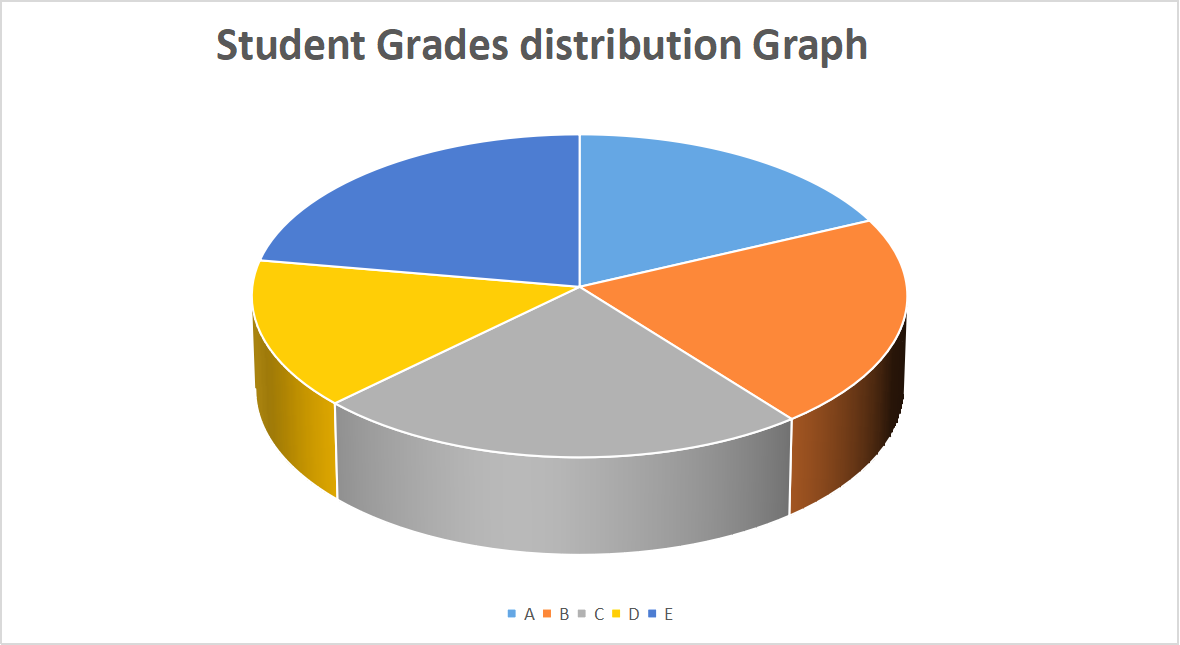
\includegraphics[width=0.7\linewidth]{img/pie_chart}
	\caption{}
	\label{fig:piechart}
\end{figure}

In this pie chart, we use five different colors to represent five different grades. The first issue is that the color selection is not appropriate, in other words, a more comparative color choices should be made to make the graph easier to understand. For instance, the yellow and orange color is not so comparative, which means you may have to remember this specific corresponding relation: "yellow represents D grade and orange represents B grade" with more extra time. 

Secondly, which is the most important issues is that comparing pie charts of different sizes could be misleading as we cannot accurately read the detailed information in this graph,especially the sample size is small and the difference between each data is small.

 
\textbf{Compute the perceputal distortion:}

Lie Factor Formula: sieze of effect shown in graphic/ size of effect in data:

To measure size of effect shown in graphic, we use the area of circle to compute the factor ge.

$$pd=\frac{ge}{de}$$
$$ge=\frac{22-14}{17+20+22+14+21}*2*\pi\approx 0.538$$
$$de=\frac{22-14}{14}=\frac{4}{7}$$
$$pd=\frac{0.538}{0.5714}\approx0.942$$

Overall, the perceptual distortion rate of this image,which is also called Lie Factor of this image is approximately 94.2\%.

\section{Some Improvement Aspects}
In this case, we want to show the distribution of different grades and some hidden information below. So replacing pie chart with bar chart can be a efficient way as it directly shows the difference between the number of students in each grades. Also comparing the length of a bar from a 2D perspective is much more easier than comparing the area or angle of a pie chart from a 3D perspective.

Also, adding detailed numbers in each subarea of pie chart can also directly shows the difference between each area.

Meanwhile, in this case which has only five different catogories, selecting comparative color combination may be easier for reader to directly understand the information.

\section{Summary}
Overall, the visualization work in this homework, mainly describes a virtual case about the distribution of grades of students. The first section i use a 3D pie chart to demonstrate the properties of these data, while seems confusing and not easy to understand compared with using bar chart. 

The second part of this homework illustrates mainly three perspectives of changing it into a good figure which is easier to understand and memorized.

\begin{figure}[h]
	\centering
	\begin{minipage}{0.49\linewidth}
		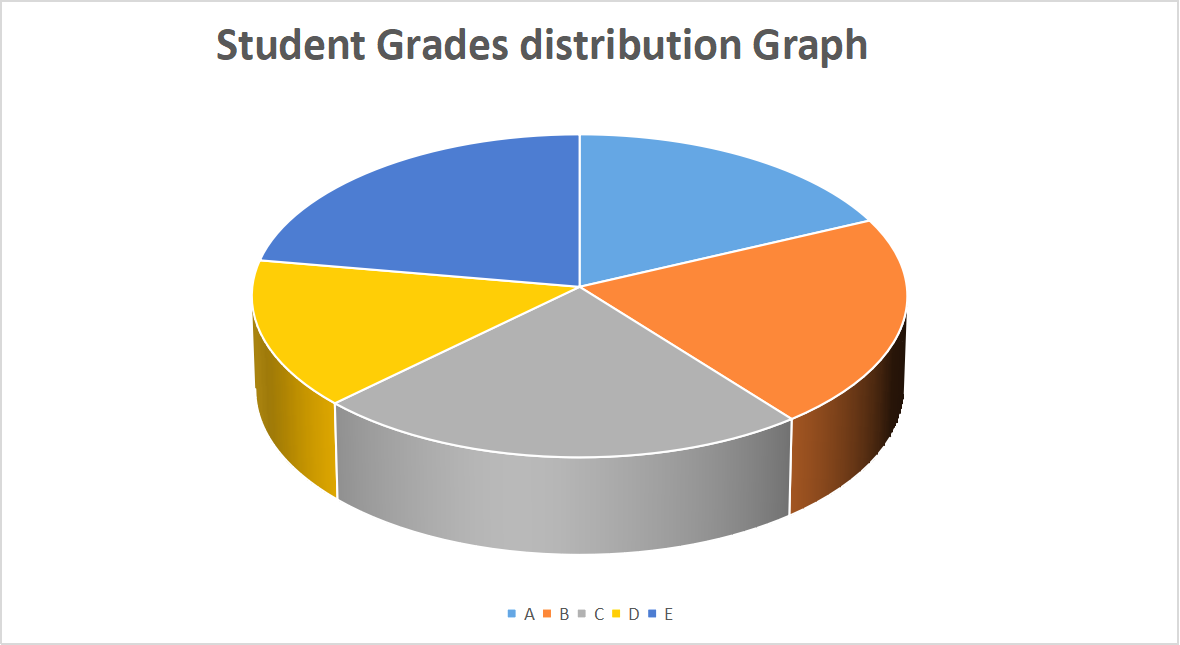
\includegraphics[width=0.9\linewidth]{img/pie_chart}
		\caption{Pie chart}
		\label{fig:piechart}
	\end{minipage}
	\begin{minipage}{0.49\linewidth}
		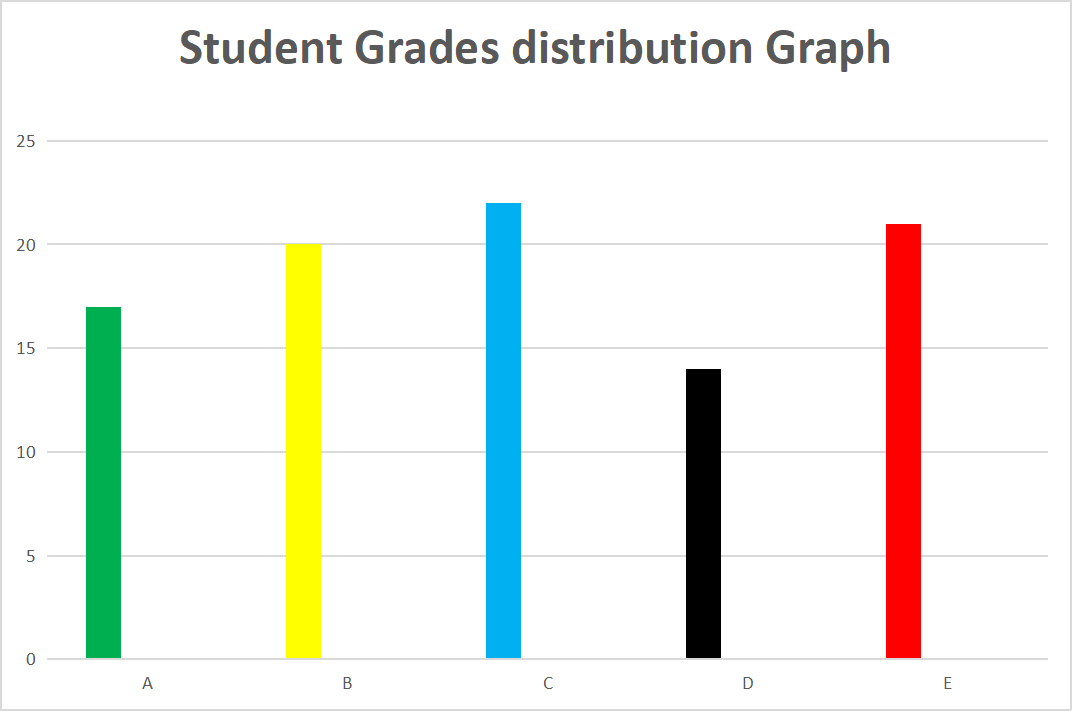
\includegraphics[width=0.9\linewidth]{img/bar_chart}
		\caption{Bar chart}
		\label{fig:piechart}
	\end{minipage}
\end{figure}



% R code here if necessary \begin{lstlisting}[style=cmd]
% load('mydata.Rdata')
% \end{lstlisting}
% \ \\

% Output of the code
% \begin{lstlisting}[style=output]
%  this is a code in output style ...
% \end{lstlisting}
% \ \\
% Code inline
% \lstinline[style=cmd]|this is an inline code ...|\\
% \ \\

% To add an image:
% 
\includegraphics[scale=0.5]{logoDMI.jpg} % save images in the folder img


